\section{弾性による高速化への影響}
\label{sec:elasticity-discussion}

\ref{sec:viscosity}章にて示した通り,超音波照射された擬塑性流体中を落下する球の高速化の要因として粘性による影響では説明が十分にできない.球の落下速度が遅い場合,粘性以外の要因によって,超音波照射による落下球の高速化が抑制されていると考えられる.そこで,本章において先行研究である岩室\cite{ref:8}にて示唆されていた弾性による影響に関して考える.

\ref{sec:elasticity}節にて,貯蔵弾性率$G'$,損失弾性率$G''$と応力$\tau$の関係性を示した.また,弾性と粘性の支配要素が変わる応力$\tau_\text{0}$も示した.この応力$\tau_\text{0}$と式(\ref{eq:tauU})によって示された,擬塑性流体中を落下する球によって生じる応力$\tau_\text{U}$の比である,$\tau_\text{U}/\tau_\text{0}$を用いて,超音波照射による球の高速化度合いを整理する.この比が1より大きいと粘性による影響が,1より小さいと弾性による影響が大きい.この整理を行うことで,弾性による超音波照射された落下球の高速化度合いへの影響を考えることができる.

応力比と高速化度合いの関係性を示した結果をFig.\ref{fig:elastcity}に示す.Fig.\ref{fig:elastcity}(a)は全ての実験結果を,Fig.\ref{fig:elastcity}(b)はPAA0.2wt.\%,岩室\cite{ref:8}以外の実験結果を示す.先行研究である岩室\cite{ref:8}の実験結果を含めた場合あまり相関が見られないが,今回の実験結果のみに限った場合,応力比1近傍にて高速化が顕著に現れた.球の落下による応力は超音波照射していない状態における終端速度にて定義されているため,超音波照射周波数や平均圧力振幅の要素を考慮していない.そのため,超音波照射周波数や平均圧力振幅の要素をパラメータとして扱っているため,弾性によって高速化を適切に整理できないと考えられる.

式(\ref{eq:muU}),(\ref{eq:muABL}),(\ref{eq:Udiff})より,終端速度$U_\text{T}$と高速化度合いの関係は,
\begin{eqnarray}
    \frac{U_\text{ABL}}{U_\text{T}} \sim U_\text{T}^{n-1} \left(\frac{1}{u}\right)^{n-1} \left(\frac{\delta}{a}\right)^n ,
    \label{eq:UTdiff_UT}
\end{eqnarray}
と見積もられる.擬塑性流体では$0<n<1$となるため,終端速度$U_\text{T}$の乗数は負となり,終端速度が小さくなると高速化がより顕著に現れると考えられる.式(\ref{eq:tauU})より,終端速度が小さくなると応力比も小さくなる.一方で,応力比が1より小さいと粘性ではなく弾性が支配的になる.ゆえに,粘性が支配的な領域では式(\ref{eq:UTdiff_UT})によって超音波照射による高速化が生じていたと考えられる.一方で,応力比が1より小さい領域では,弾性が支配的となり,粘性によって生じる超音波照射による高速化が抑制されたと考えられる.よって,終端速度が小さく,弾性が支配的とならない応力比が1近傍で高速化が顕著に現れたと考えられる.

超音波照射による高速化に対する,粘性と弾性の影響を考慮するため,横軸を粘性による影響,縦軸を応力比とし,高速化度合いをカラーバーで示した結果をFig.\ref{fig:elastcityColor}に示す.

\begin{figure}[h]
    \centering
    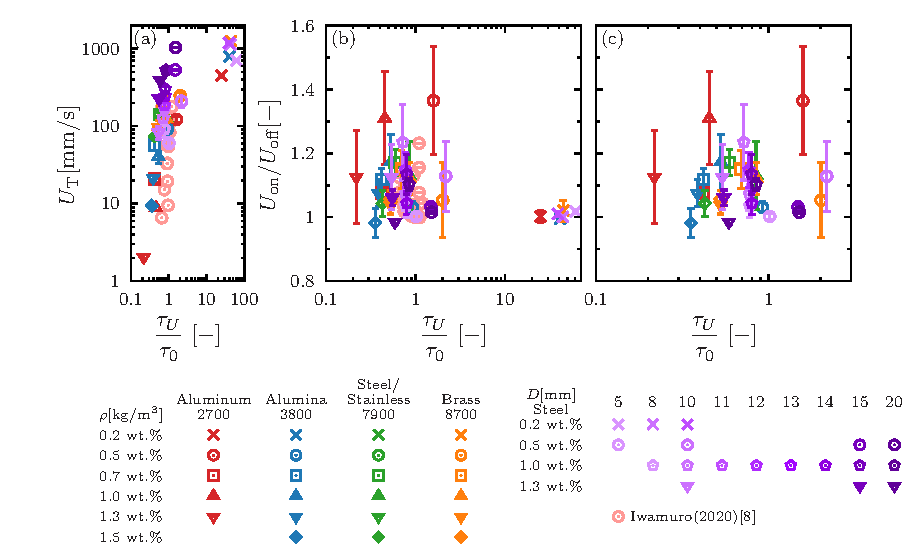
\includegraphics[width=0.9\textwidth]{5-Results/elastcity.eps}
    \caption{Relationship between velocity ratio and elasticity ratio $\tau_\text{U}/\tau_\text{0}$ by (a)all experiment, (b)without PAA0.2wt.\%.}
    \label{fig:elastcity}
\end{figure}

\begin{figure}[h]
    \centering
    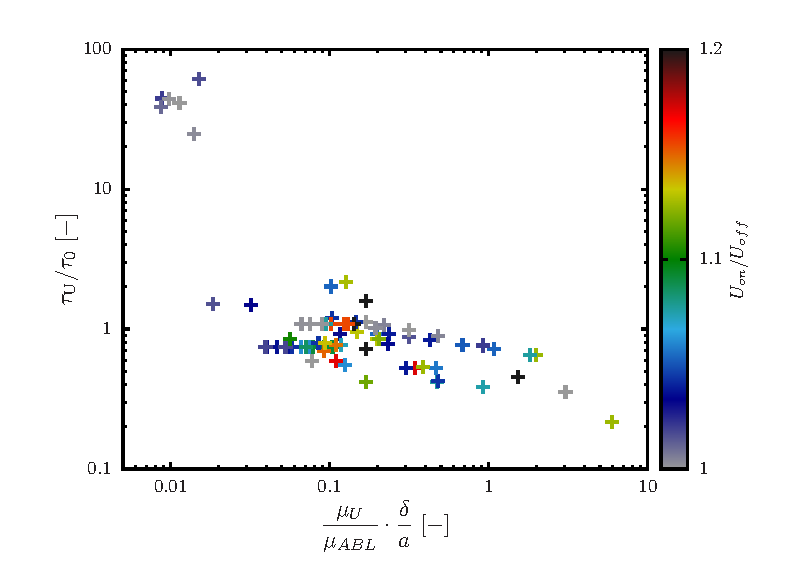
\includegraphics[width=0.9\textwidth]{5-Results/elastcity_color.eps}
    \caption{}
    \label{fig:elastcityColor}
\end{figure}
